\chapter{Namuru}\label{ch:Namuru}

\section{\ac{GNSS} Receivers}

\ac{GNSS} Receivers use trilateration to position a receiver using signals transmitted from a constellation of satellites. The range to from each satellite to the receiver (pseudorange) is computed based on the time of arrival of the signal transmitted by each satellite. 

While the work in this thesis is generalisable to other \ac{GNSS}s, for example Galileo and GLONASS, this thesis will focus on tracking of the GPS L1 \ac{C/A} signal (1575.42 MHz).\ac{GPS} uses a type of \ac{CDMA} called \ac{DSSS} in order to transmit data, allowing all the satellites in the constellation to transmit on the same frequency without interference \cite{Ublox}. Additionally, the use of \ac{CDMA} allows the signal, which is typically 30dB below the thermal noise floor to be recovered\cite{Gleason,Tsui}.

The sequence used in the \ac{DSSS} modulation is called a \ac{PRN} and unique to each satellite. In order to recover the signal from a satellite, the GPS receiver correlates the incoming signal with a local replica of the \ac{PRN}. The sequence has a period of 1ms, and a tracking loop is used to maintain the code phase of a local replica, with respect to the received signal. 

Another tracking loop is used to track the incoming carrier frequency of the signal. Due to the relative motion of the satellite and the receiver, there is a difference doppler shift between the nominal transmission frequency of 1575.42 MHz and the received frequency. 

If both the carrier frequency tracking loop, and the code phase loop are working, then the signal can be de-spread, and the \ac{BPSK} data can be recovered from the signal using a \ac{PLL}.


\begin{figure}[!htb] 
    \centering
    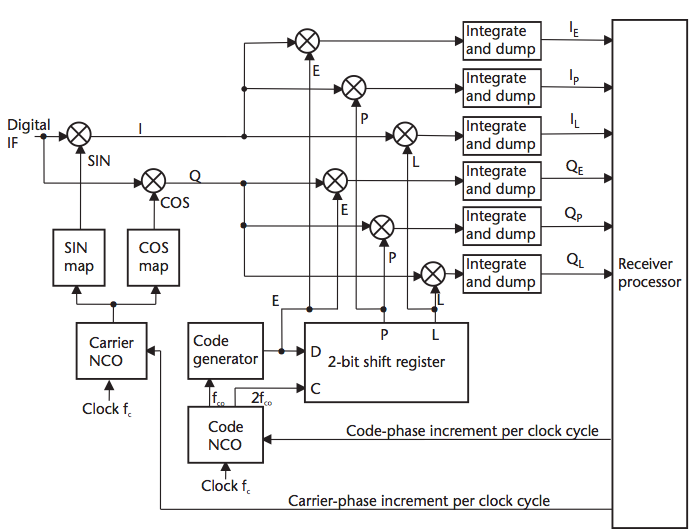
\includegraphics[width=1\textwidth]{Namuru/KaplanArchitecture2.png} 
    \caption{A generic baseband processor. In Namuru, this is implemented on a \ac{FPGA}. Note in the diagram, that the processor (microcontroller) takes samples ($I_E$,$I_P$,$I_L$,$Q_E$,\ldots) and determines the Code-phase increment and the Carrier phase increment. Image from \cite{Kaplan}.}
    \label{fig:KaplanArchitecture}
\end{figure}

\section{Namuru}

\subsection{Hardware}

\subsection{Software}

\begin{figure}[!htb] 
    \centering
    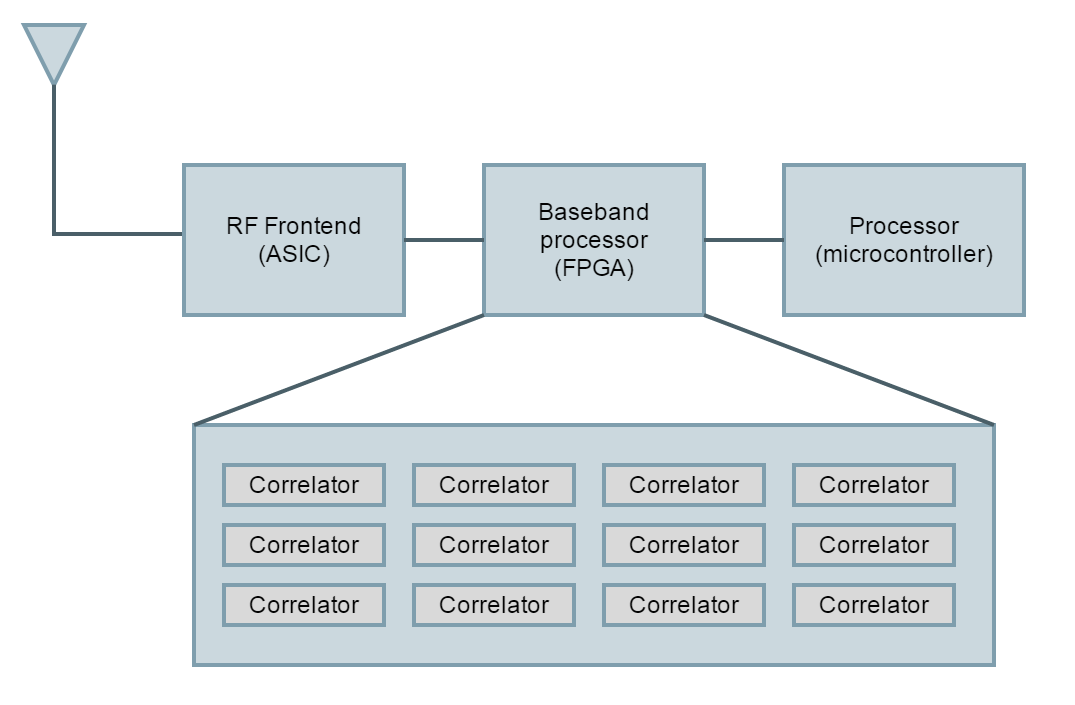
\includegraphics[width=1\textwidth]{Namuru/RecieverDiagram.png} 
    \caption{A high level diagram of the Namuru architecture. An RF font end digitises the GPS signal, this is then de-spread to baseband by a bank of 12 correlators implemented on a FPGA. The correlators are controlled by a microcontroller,which is implemented as a soft-core processor on the FPGA.}
    \label{fig:RecieverDiagram}
\end{figure}

In order to properly understand the architecture of the Namuru receiver, it is important to first understand the context which shaped it's design. \ac{GNSS} receivers use an \ac{ASIC} RF front-end to convert the \ac{RF} signal from the satellite to a digitised \ac{IF} signal which can then be de-spread to baseband by the correlators. 

An \ac{ASIC} front-end consists of the following components \cite{GlennonPresentation}: 

\begin{itemize}
\item{\ac{LNA} to amplify signal from antenna}
\item{\ac{PLL} to generate a local oscillator}
\item{Mixers to down-convert RF signals to IF}
\item{\ac{LPF} for image rejection}
\item{\ac{AGC} to maximise dynamic range}
\item{\ac{ADC} to digitise signal}
\end{itemize}

The architecture of a typical \ac{GNSS} \ac{RF} front-end can be found in figure \ref{fig:Zarlink2015}.  

\begin{figure}[!htb] 
    \centering
    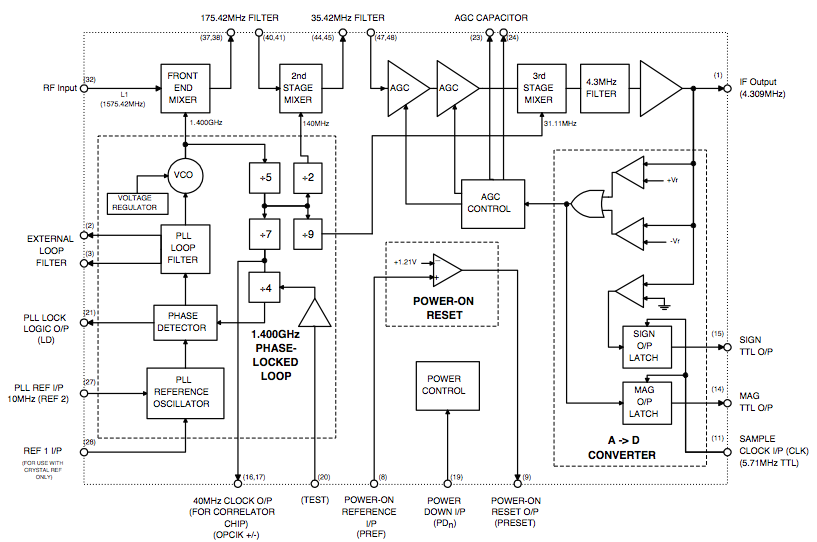
\includegraphics[width=1\textwidth]{Namuru/Zarlink2015.png} 
    \caption{The architecture of the Zarlink GP2015 \ac{RF} front-end. Image from \cite{Zarlink2015}}
    \label{fig:Zarlink2015}
\end{figure}

In a commercial design, the RF front-end is coupled with an \ac{ASIC} baseband processor. The use of an \ac{ASIC} chip-set is problematic, as historically, most \ac{GNSS} chip-sets come with firmware supplied as pre-compiled binary images \cite{Glennon11aquariusfirmware}. 
Additionally, manufacturers generally do not publish datasheets that describe the operation of the baseband correlator\cite{Glennon11aquariusfirmware}. Finally the supply of GPS chipsets has become significantly more constrained, acting as a disincentive to the use of chipsets for research.

A solution to this problem, which is popular with academic institutions is the use of \ac{SDR} for the development of receivers. \ac{IF} data is captured using an \ac{SDR}, and processed in software\cite{Glennon11aquariusfirmware}, One example of a MATLAB software receiver is described in \cite{KaiBorre}.

The key drawback of this approach is processing speed, because the correlation occurs in software, rather than specialised hardware. Optimised software coupled with powerful hardware is required to carry out process the \ac{IF} data in real time. The use of powerful hardware to carry out the correlation in software results in a solution that is not cost effective and suffers from excessive power consumption.

The development of a \ac{FPGA} digital baseband processor represents an elegant compromise. 
The architecture of the Namuru receiver can be found in figure \ref{fig:RecieverDiagram}. The receiver contains an \ac{ASIC} front end, a \ac{FPGA} baseband processor, and a microcontroller processor, which controls the tracking loops in the \ac{FPGA}, and computes a navigation solution. In some versions of the Namuru receiver, the processor has been a soft core processor, implemented on the \ac{FPGA}.

This digital \ac{IF} signal is processed by a \ac{FPGA} digital baseband processor which contains 12 hardware correlators. The correlators are used to de-spread the signal and recover the navigation data using a \ac{PLL}.

\section{Tracking Loops}
In order to recover the data message, a \ac{GNSS} receiver needs to simultaneously track:

\begin{itemize}
\item{The \ac{PRN} code phase, using a \ac{DLL}} 
\item{The carrier phase, using a \ac{PLL}}
\end{itemize}

\subsection{Code loop}

\subsection{Carrier loop}


Before phase lock can be achieved, the frequency of the local signal must be relatively close to frequency of the incoming signal from the satellite. Hence a \ac{FLL} is often used to sufficiently reduce the frequency error between the local signal and the received signal.

The code phase changes with the range to the satellite while the carrier frequency changes around the centre frequency of 1575.42 MHz due to the doppler effect\cite{Tsui}.

The frequency offset due to the \ac{LOS} velocity between the receiver and the satellite can be found as : 

\begin{equation}
\Delta f = f_0\frac{v}{c}
\end{equation}

Where: 
\begin{framed}
\begin{align*}
f_0 &= 1575.42 MHz\\   
c &= 2.99792458 \times 10^8
\end{align*}
\end{framed}

For the GPS L1 \ac{C/A} signal, this results in a shift of 5.25Hz per m/s. 
While the receiver is stationary, there will still be a doppler shift, of up to 20KHz due to the motion of the satellite\cite{Kaplan}. As the receiver moves, there will be an doppler shift due to the change in the \ac{LOS} distance between the satellite and the receiver, resulting in a constant offset, for a constant velocity. If the receiver undergoes a constant acceleration, then the doppler frequency increases as a ramp. The relationship between different derivatives of position, and the doppler frequency produced is in table \ref{table:DopplerDynamics} for reference.

Understanding how the Doppler frequency changes is crucial when designing tracking loops, which shall be discussed in more detail in the literature review. 

A thorough overview of the dynamics experienced during space flight can be found in Appendix 1.
\begin{table}[!htb]
\centering
\begin{tabular}{|l|l|}
\hline
\rowcolor[HTML]{C0C0C0} 
Change in \ac{LOS} Distance & Doppler frequency \\ \hline
Static                 & 0                 \\ \hline
\rowcolor[HTML]{EFEFEF} 
Velocity               & Constant          \\ \hline
Acceleration           & Ramp              \\ \hline
\rowcolor[HTML]{EFEFEF} 
Jerk                   & Parabolic         \\ \hline
\end{tabular}
\caption{The relationship between \ac{LOS} dynamics and Doppler frequency}
\label{table:DopplerDynamics}
\end{table}


The dynamics experienced by the code tracking loop are 1540 times smaller than those experienced by the carrier loop \cite{Kaplan}. Hence the  code loop is significantly more robust than either the \ac{FLL} or \ac{PLL}.

The \ac{PLL} is the most vulnerable of the loops, and under extreme dynamics, the \ac{PLL} will break while the \ac{FLL} will keep tracking, before the \ac{PLL} resumes tracking once the dynamics have subsided to more reasonable levels. If the \ac{PLL} looses phase lock, then the receiver is unable to continue receiving the data signal from the satellite, and hence the receiver is unable to continue providing position solutions. Because of the venerability of the \ac{PLL} to dynamics,the analysis and design of \ac{PLL}'s for high dynamics it will be the focus of this thesis. 
